\documentclass[12pt]{article}
\setlength{\textwidth}{17cm}
\setlength{\textheight}{24cm}
\setlength{\topmargin}{-2cm}
\setlength{\footskip}{1cm}
\setlength{\evensidemargin}{0cm}
\setlength{\oddsidemargin}{0cm}
\setlength{\parindent}{0cm}

\usepackage{allrunes}
\usepackage{amsmath}
\usepackage[magyar]{babel}
\usepackage[T1]{fontenc}
\usepackage[utf8]{inputenc}
\usepackage{fixltx2e}
\usepackage{multirow}

\usepackage[hyphens]{url}
\usepackage[unicode,colorlinks=true,breaklinks]{hyperref}
%\usepackage[dvips]{hyperref}
%should display links, but it does not work with \H accent
%and formulas in section titles

\hypersetup{colorlinks,linkcolor=blue,urlcolor=magenta,citecolor=magenta}
%Breaks long url`s in text, while keeping it one link:

\usepackage{amsfonts}
\usepackage{amsthm}
\usepackage{amssymb}


\theoremstyle{plain}
\usepackage{graphicx}

%\usepackage{gensymb}
\usepackage{float}

% For bra-ket notation
\usepackage{braket}

%% New commands
\newcommand{\dd}{\textrm{d}}

%% Pauli matrices
\newcommand{\sigx}{\sigma_x}
\newcommand{\sigy}{\sigma_y}
\newcommand{\sigz}{\sigma_z}

\newcommand{\paulix}{
    \left( \begin{array}{cc}
        0 & 1 \\
        1 & 0
    \end{array}
    \right)
}

\newcommand{\pauliy}{
    \left( \begin{array}{cc}
        0 & -i \\
        i & 0
    \end{array}
    \right)
}

\newcommand{\pauliz}{
    \left( \begin{array}{cc}
        1 & 0 \\
        0 & -1
    \end{array}
    \right)
}

% \begin{figure}[H]
%     \begin{center}
%     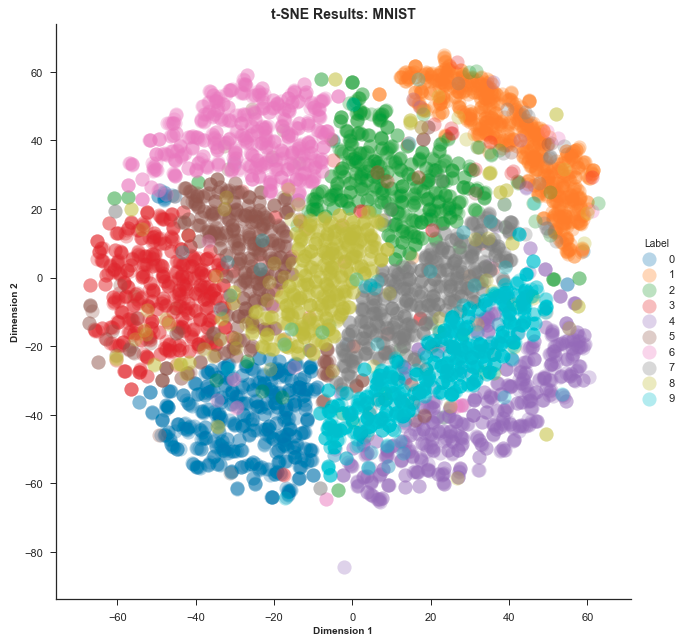
\includegraphics[width=0.5\textwidth]{media/tsneplot.png}
%     \caption{t-SNE plot for MNIST dataset \cite{tsne-article}} 
%     \label{fig:tsneplot}
%     \end{center}
% \end{figure}

\begin{document}
\title{\textbf{11. tétel}}
\author{Berekméri Evelin}

\maketitle


\newpage
\begin{abstract}

Számítógépes tanulás – Predikciós és klasszifikációs módszerek. Felügyelt és felügyelet nélküli tanítás. A tanítóhalmaz, a validáció és a túlfittelés. K-means, Support Vector Machine, Random Forest, k-NN-módszer.
\end{abstract}

\section*{Klasszifikációs módszerek}
Klasszifikáció során kvalitatív válaszokat prediktálunk, amelyek egy véges halmazból vesznek fel értékeket. %Prediktálhatjuk először annak a valószínűségét is, hogy melyik halmazba tartozik egy érték, akkor ezek a módszerek is regresszióként működnek.
Klasszifikációs módszerek: logisztikus regresszió, lineáris diszkriminancia-analízis, KNN, tree, random forest, boosting, support vector machine. 

\section*{Felügyelt és felügyelet nélküli tanítás}
Felügyelt tanítás esetén egy statisztikai modellt építünk inputok alapján azért, hogy prediktáljuk vagy megbecsüljük az outputokat. Minden megfigyeléshez ($x_i$ "predictor" érték(ek)hez) tartozik egy $ y_i $ "válasz" érték.  Ilyen módszerek például a lineáris és logisztikus regresszió, boosting, support vector machine.  

Felügyelet nélküli tanulás során nincsenek outputok, csak inputok, amik alapján az adathalmaz szerkezetéről és kapcsolatairól tudhatunk meg többet. Ilyen módszer például a klaszterezés. 

\section*{A tanítóhalmaz, a validáció és a túlfittelés}
A rendelkezésünkre álló adathalmazt felosztjuk tanítóhalmazra, validációs halmazra és teszthalmazra. 

\section*{K-means, Support Vector Machine, Random Forest, k-NN-módszer}

\begin{thebibliography}



\end{thebibliography}

\end{document}